\chapter{Laws of Nature, Four-Vectors, and Tensors}

This lecture is not really about entanglement in the narrow sense. It is about the form that laws of nature are allowed to take. Following Leonard Susskind's order of attack, and curated here by LazyingArt LLC, we begin with a deliberately bad law, repair it by demanding invariance under rotations and then under Lorentz transformations, and only after that introduce the notation of four-vectors, scalars, and tensors. Throughout most of the chapter we set \(c=1\); when useful, we briefly restore \(c\) to make the low-velocity limit transparent.

\section{Symmetry As The First Test Of A Law}

Susskind begins in the right place: not with formalism, but with an example that is mathematically possible and physically wrong. Suppose we invent a law saying that two particles interact whenever their \(x\)-coordinates become equal. There is no contradiction in such a rule. One can write
\begin{equation}
x_1-x_2=0.
\end{equation}
If that condition holds, the particles may bounce, turn around, or fly off in some new direction. Nothing prevents us from imagining such a world.

But already one feels that the law has the wrong shape. It refers to one coordinate component as though nature cared about the way we happened to orient the blackboard. That discomfort is the point of the example. The lecture is asking what is wrong, not dynamically, but structurally.

\subsection{Question \& Answer}

\paragraph{What symmetry is actually being violated?}

A student answers: homogeneity of space. Susskind's correction matters, and it should be preserved. The law does \emph{not} violate homogeneity. It does not single out any preferred value of \(x\); if we translate the whole configuration, the statement \(x_1-x_2=0\) remains the same. Translation invariance survives.

What fails is isotropy. If we rotate the axes by \(90^\circ\), the same physical rule would have to say that particles interact when their \(y\)-coordinates are equal. The law has changed form under a rotation. That is the real defect. One may use many coordinate systems, but the laws of physics should not owe their simplicity to an arbitrary choice of axis.

This is the opening moral of the lecture: a law of nature is not merely something true in one coordinate system. It should be written in a form that survives a change of coordinates.

\section{From Spatial Coincidence To Spacetime Coincidence}

The repair comes immediately. Instead of requiring equality of one component, we require equality of position itself. In two or three dimensions, the particles interact only when they arrive at the same point in space. If \(\vec r_1\) and \(\vec r_2\) are their position vectors, the collision rule becomes
\begin{equation}
\vec r_1=\vec r_2,
\qquad\text{or equivalently}\qquad
\vec r_1-\vec r_2=\vec 0.
\end{equation}
This is now a vector equation. It says that the \emph{whole} separation vector vanishes. And that is precisely the kind of statement that survives a rotation. A vector that is zero in one coordinate system is zero in any rotated coordinate system. Likewise, if two vectors are equal in one frame, they are equal in every rotated frame.

Susskind pauses on this point because it is the real reason we like vector equations. A single component of a vector may happen to vanish in one frame and not in another. But the statement that an entire vector vanishes is coordinate-independent. That is why physics is naturally written in terms of whole transforming objects rather than isolated pieces of them.

Only then does he bring time back in. One might try a Newtonian-looking law saying that collisions occur when the times of two particles are equal. In pre-relativistic physics that is perfectly sensible. In relativity it is not. Simultaneity is frame-dependent, so a condition on the time component alone cannot define a relativistic law.

The same logic that repaired the spatial law now repairs the spacetime law. A spacetime vector may have zero spatial components and still fail to vanish:
\[
\Delta X^\mu=(0,0,0,\Delta t)\neq 0.
\]
So it is not enough to say that the spatial parts agree. For a relativistic collision, the two events must coincide as a \emph{whole} spacetime event. If \(X^\mu\) denotes the spacetime position of an event, then the simple collision rule is
\begin{equation}
X_1^\mu=X_2^\mu,
\qquad\text{or}\qquad
X_1^\mu-X_2^\mu=0.
\end{equation}
This is the bridge from ordinary vectors to four-vectors. The lecture is still teaching one lesson, now in a larger arena: laws must be written in terms of entire objects that transform coherently.

\section{Four-Vectors And Matrix Form Of Transformations}

A four-vector is an object whose components transform exactly as the coordinates of spacetime do. In the lecture the index convention is \((1,2,3,0)\), with \(0\) reserved for time. Thus we may write
\[
X^\mu=(x^1,x^2,x^3,x^0)=(x,y,z,t).
\]

Susskind first recalls explicit examples. For a boost in the \(x\)-direction, the cleaned standard form is
\begin{align}
x'&=\gamma(x-vt),&
y'&=y,&
z'&=z,&
t'&=\gamma(t-vx),
\end{align}
with
\begin{equation}
\gamma=\frac{1}{\sqrt{1-v^2}}.
\end{equation}
The transcript around the board formulas is noisy, but the intended content is secure.

He then turns to ordinary spatial rotations. For a rotation about the \(z\)-axis, the lecture again gives a linear transformation, mixing \(x\) and \(y\) while leaving \(z\) and \(t\) alone. In cleaned form,
\begin{equation}
\begin{pmatrix}
x'\\
y'\\
z'\\
t'
\end{pmatrix}
=
\begin{pmatrix}
\cos\theta & \sin\theta & 0 & 0\\
-\sin\theta & \cos\theta & 0 & 0\\
0 & 0 & 1 & 0\\
0 & 0 & 0 & 1
\end{pmatrix}
\begin{pmatrix}
x\\
y\\
z\\
t
\end{pmatrix}.
\end{equation}
Here too we are normalizing the lecture to the standard \(z\)-axis rotation matrix, since the transcript around the explicit coefficients is partially garbled.

The crucial point is not the details of any one matrix. The crucial point is that boosts and rotations are both \emph{linear}. Their more general combinations are obtained by multiplying matrices together, and the order matters. Susskind even pauses to note that rotating and then boosting is not the same as boosting and then rotating. The transformations form a structured family, not a random collection of coordinate tricks.

\begin{figure}
\centering

\includegraphics[width=0.68\textwidth]{lecture_06_figure_03.png}
\caption{Indexed Lorentz transformation and the beginning of its column-vector form on the board.}
\end{figure}

The board then makes the decisive move from explicit component formulas to compact notation. The legible indexed law is
\begin{equation}
X'^{\mu}=L^{\mu}{}_{\nu}X^{\nu}.
\end{equation}
This is the same matrix multiplication rule written with indices. The repeated index \(\nu\) is understood to be summed over. That is the Einstein summation convention, and it is nothing more mysterious than the ordinary rule for multiplying a matrix by a column vector.

The lower line in the frame is only partially written, so the full column-vector form is a cautious standard reconstruction:
\begin{equation}
\begin{pmatrix}
x'\\
y'\\
z'\\
t'
\end{pmatrix}
=
L
\begin{pmatrix}
x\\
y\\
z\\
t
\end{pmatrix}.
\end{equation}
This pairing of the indexed law with the column-vector law is exactly the pedagogical point of the board. The lecture is showing us two ways of writing the same transformation.

From here the general definition becomes clear. A quantity \(A^\mu\) is a four-vector if it transforms in the same way as spacetime position:
\begin{equation}
A'^{\mu}=L^{\mu}{}_{\nu}A^{\nu}.
\end{equation}
And with that in hand we can write laws in two equivalent styles: either a whole four-vector is set equal to zero, or one whole four-vector is set equal to another. What is never acceptable is to write laws for disconnected pieces of a four-vector and then hope Lorentz invariance will somehow survive.

\section{Scalars, Lowered Indices, And Invariants}

At this stage Susskind deliberately slows down. Before going farther with four-vectors, he says, we should really have talked about scalars first. That is an important pedagogical beat. A scalar is a quantity that does not change under the transformation in question. Under rotations, temperature at a point is a scalar. The distance between two points in space is also a scalar.

He even gives a deliberately silly example: the distance between two points might happen, numerically, to equal the temperature in the room. Precisely because both quantities are scalars, the statement is rotationally invariant. Its truth does not depend on how we orient the axes. The example is silly, but the lesson is serious: invariant statements can be made out of invariant objects.

Vectors are different. Their components change from one frame to another. So we need a way to combine components into quantities that do \emph{not} change.

Let \(A^\mu\) be a general four-vector. Its contravariant components are written with the index upstairs. The same geometric object can also be described by covariant components, written with the index downstairs. The connection is made by the Minkowski metric:
\begin{equation}
A_{\mu}=\eta_{\mu\nu}A^{\nu},
\qquad
\eta_{\mu\nu}=
\begin{pmatrix}
-1&0&0&0\\
0&-1&0&0\\
0&0&-1&0\\
0&0&0&1
\end{pmatrix}.
\end{equation}
With the sign convention used throughout this lecture, lowering the index changes the signs of the three spatial components and leaves the time component unchanged:
\[
A^\mu=(A^1,A^2,A^3,A^0)
\qquad\Longrightarrow\qquad
A_\mu=(-A^1,-A^2,-A^3,A^0).
\]
The transcript briefly wobbles between \(0\) and \(4\) for the time component, and Susskind corrects an index slip on the board. In the notes we simply standardize on \(0\).

Now we can see why lowering the index is useful. It lets us form invariant quadratic expressions in a compact way:
\begin{equation}
A_{\mu}A^{\mu}
=
-\left(A^1\right)^2-\left(A^2\right)^2-\left(A^3\right)^2+\left(A^0\right)^2.
\end{equation}
For the spacetime position vector this becomes
\begin{equation}
X_{\mu}X^{\mu}=t^2-x^2-y^2-z^2.
\end{equation}
This is the invariant interval. It is the relativistic analogue of a length, with the crucial sign difference between space and time built in.

There is also a notational principle here. Whenever we sum over a repeated index, one copy should be upstairs and the other downstairs. Susskind emphasizes this before even explaining all of its consequences. In this notation, the very form of the equation is already steering us toward invariant combinations.

The next step is the bilinear product of two four-vectors. If \(A^\mu\) and \(B^\mu\) are four-vectors, then
\begin{equation}
A_{\mu}B^{\mu}
\end{equation}
is also invariant. The lecture's proof is elegant and worth preserving. Since sums and differences of four-vectors are again four-vectors, the quantities
\[
(A+B)_\mu(A+B)^\mu
\qquad\text{and}\qquad
(A-B)_\mu(A-B)^\mu
\]
must both be invariant. Expanding gives
\begin{align}
(A+B)_\mu(A+B)^\mu&=A_\mu A^\mu+B_\mu B^\mu+2A_\mu B^\mu,\\
(A-B)_\mu(A-B)^\mu&=A_\mu A^\mu+B_\mu B^\mu-2A_\mu B^\mu.
\end{align}
Subtracting one from the other isolates the cross term:
\begin{equation}
(A+B)_\mu(A+B)^\mu-(A-B)_\mu(A-B)^\mu=4A_\mu B^\mu.
\end{equation}
The left-hand side is a difference of invariants, so \(A_\mu B^\mu\) must itself be invariant. This is the relativistic inner product. Apart from the sign structure supplied by \(\eta_{\mu\nu}\), it plays the role that the dot product plays for ordinary vectors.

\section{Proper Velocity And Four-Momentum}

Only after that notational groundwork does the lecture return to a concrete physical four-vector: the infinitesimal displacement along a worldline,
\[
dx^\mu=(dx,dy,dz,dt).
\]
Its invariant norm defines the proper time:
\begin{equation}
d\tau^2=dx_\mu dx^\mu=dt^2-dx^2-dy^2-dz^2.
\end{equation}
Then the proper four-velocity is defined by
\begin{equation}
u^\mu=\frac{dx^\mu}{d\tau}.
\end{equation}
This is already a physically important shift. Ordinary velocity is \(d\vec x/dt\). Proper velocity is the rate of change of spacetime position with respect to the particle's own proper time.

The lecture immediately points out that \(u^\mu\) has four components, which seems strange at first. But they are not independent. In fact,
\begin{equation}
u_\mu u^\mu
=
\frac{dx_\mu dx^\mu}{d\tau^2}
=
\frac{d\tau^2}{d\tau^2}
=
1.
\end{equation}
So the four-velocity is a unit timelike four-vector. The fourth component is fixed by the first three, just as the components of an ordinary unit vector are constrained by its length.

\paragraph{Worked derivation.}
To connect proper velocity with ordinary velocity, we examine the spatial components:
\begin{equation}
u^i=\frac{dx^i}{d\tau}
=
\frac{dx^i}{dt}\frac{dt}{d\tau}
=
v^i\frac{dt}{d\tau}.
\end{equation}
Now divide the defining equation for \(d\tau^2\) by \(dt^2\):
\begin{equation}
\left(\frac{d\tau}{dt}\right)^2
=
1-\frac{dx^2+dy^2+dz^2}{dt^2}
=
1-\frac{v^2}{c^2}.
\end{equation}
Therefore
\begin{equation}
\frac{dt}{d\tau}
=
\frac{1}{\sqrt{1-v^2/c^2}}
=
\gamma.
\end{equation}
Hence
\begin{equation}
u^i=\gamma v^i,
\qquad
u^0=\frac{dt}{d\tau}=\gamma.
\end{equation}
The lecture carefully addresses a possible confusion here. This \(\gamma\) is the same mathematical function that appears in Lorentz boosts, but now its argument is the speed of a particle in a chosen frame, not the relative speed between two inertial frames. It is the same function, used in a different context.

For small velocities, \(\gamma\approx 1\). Then the first three components of \(u^\mu\) are close to the ordinary velocity, and the time component is close to \(1\) in the \(c=1\) convention. As the particle speed approaches the speed of light, all components grow large.

Momentum is introduced in exactly the same spirit. Ordinary \(m\vec v\) is not a four-vector, because ordinary \(\vec v\) is not a four-vector. The relativistically natural definition is
\begin{equation}
p^\mu=mu^\mu.
\end{equation}
This is the four-momentum. In components,
\[
p^\mu=(\gamma mv_x,\gamma mv_y,\gamma mv_z,\gamma m)
\]
when \(c=1\). The first three components reduce to ordinary momentum at low speed. The last component is the energy component; with \(c\) restored, it contains the familiar rest energy together with the kinetic correction. The lecture does not yet dwell on that relation, but it keeps the connection with ordinary mechanics clearly in view.

\section{The Puzzle In The Lorentz Force Law}

At this point Susskind says, in effect, let us take a vacation from relativity and write the old law first. That turn in the lecture matters. The point is not to derive the relativistic force law immediately, but to see precisely why the pre-relativistic form cannot be fundamental.

He briefly notes that if one wanted a four-dimensional acceleration, the natural guess would be the proper-time derivative of four-velocity. But he deliberately does not push that construction yet. First he writes the familiar law of motion for a charged particle:
\begin{equation}
\vec F=q\left(\vec E+\vec v\times\vec B\right).
\end{equation}
The electric part is velocity-independent. The magnetic part depends explicitly on the particle's velocity. This is exactly where the trouble begins.

\subsection{Question \& Answer}

\paragraph{If the particle is at rest in one frame, where can the force come from?}

Suppose that in one frame there is only a magnetic field. Then the force comes entirely from the term \(q\,\vec v\times\vec B\). Now move to the instantaneous rest frame of the particle. In that frame \(\vec v=0\), so the magnetic contribution disappears. But the particle was accelerating. A mere change of frame cannot make a genuine acceleration vanish. Therefore the new frame must contain an electric field, and that electric field must account for the force.

This is the lecture's conceptual turning point. What one observer calls a purely magnetic field cannot remain purely magnetic in every frame. Electric and magnetic fields must mix under Lorentz transformations. The decomposition into \(\vec E\) and \(\vec B\) is not invariant; it is frame-dependent.

So what do we need? We need an object with six components altogether, one that can mix these six quantities in a coherent Lorentz-covariant way. It is not a scalar, and it is not a four-vector. Something new has to appear.

\section{Tensors, Symmetric Versus Antisymmetric, And The Field Tensor Preview}

The need for that new object is what brings tensors into the lecture. Only after the six-component problem is on the table does Susskind introduce them. A scalar is a tensor of rank zero. A four-vector is a tensor of rank one. A rank-two tensor has two indices. The simplest examples on the board are
\begin{equation}
A^\mu B^\nu,
\qquad
A^\mu B^\nu C^\sigma.
\end{equation}
The first is rank two; the second is rank three.

\begin{figure}
\centering

\includegraphics[width=0.72\textwidth]{lecture_06_figure_05.png}
\caption{Rank-two tensor notation and the schematic component grid used on the board to discuss independent entries.}
\end{figure}

The frame is valuable because it preserves exactly the board logic: abstract index notation on the left, component-array thinking on the right. A rank-two tensor in four dimensions has \(4\times4=16\) components, and we can display them as a \(4\times4\) matrix-like grid.

But a tensor is not defined by being literally a product of vectors. It is defined by how it transforms. If \(T^{\nu\tau}\) is a second-rank tensor, then
\begin{equation}
T'^{\mu\sigma}=L^{\mu}{}_{\nu}L^{\sigma}{}_{\tau}T^{\nu\tau}.
\end{equation}
There is one transformation matrix for each index. This is the operative pattern. Products of vectors transform this way, but so do sums of such products, and more general objects as well. What matters is the transformation law.

Among rank-two tensors, two special cases are singled out. A symmetric tensor obeys
\begin{equation}
T^{\mu\nu}=T^{\nu\mu},
\end{equation}
while an antisymmetric tensor obeys
\begin{equation}
T^{\mu\nu}=-T^{\nu\mu}.
\end{equation}
For a symmetric \(4\times4\) tensor, the entries reflected across the diagonal are equal. Hence the diagonal plus one triangular half determine the whole object. That gives
\begin{equation}
4+6=10
\end{equation}
independent components, exactly as the lecture says.

\begin{figure}
\centering
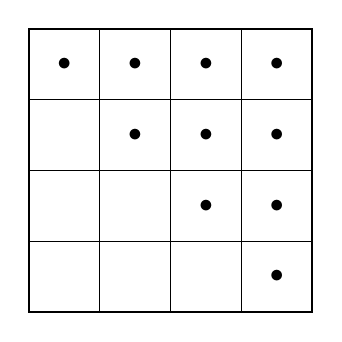
\begin{tikzpicture}[scale=0.9]
\draw[thick] (0,0) rectangle (4,4);
\foreach \x in {1,2,3} {
  \draw (\x,0) -- (\x,4);
}
\foreach \y in {1,2,3} {
  \draw (0,\y) -- (4,\y);
}
\foreach \x/\y in {
  0.5/3.5, 1.5/3.5, 2.5/3.5, 3.5/3.5,
  1.5/2.5, 2.5/2.5, 3.5/2.5,
  2.5/1.5, 3.5/1.5,
  3.5/0.5
} {
  \node at (\x,\y) {$\bullet$};
}
\end{tikzpicture}
\caption{A schematic symmetric \(4\times4\) tensor. The diagonal and one triangular half contain the ten independent components.}
\end{figure}

For an antisymmetric tensor, the diagonal must vanish, because \(T^{\mu\mu}=-T^{\mu\mu}\). The remaining independent entries occupy only one triangular half of the matrix, so there are
\begin{equation}
6
\end{equation}
independent components. That is exactly the number of components carried together by \(\vec E\) and \(\vec B\).

This is the answer to the six-component problem. The electromagnetic field is packaged into an antisymmetric tensor \(f_{\mu\nu}\). The secure identifications in the lecture are
\begin{equation}
E_1=f_{10},
\qquad
E_2=f_{20},
\qquad
E_3=f_{30},
\end{equation}
together with the cyclic magnetic pattern
\begin{equation}
f_{12}=-B_3,
\qquad
f_{23}=-B_1,
\qquad
f_{31}=-B_2.
\end{equation}
Thus the electric field occupies the slots involving the time index \(0\), while the magnetic field occupies the purely spatial slots.

The exact sign convention in the full \(4\times4\) matrix should be checked once more against the full board before the final typesetting pass, but the qualitative structure is clear. A cautious first-pass form consistent with the transcript is
\begin{equation}
f_{\mu\nu}\approx
\begin{pmatrix}
0 & -B_3 & B_2 & E_1\\
B_3 & 0 & -B_1 & E_2\\
-B_2 & B_1 & 0 & E_3\\
-E_1 & -E_2 & -E_3 & 0
\end{pmatrix}.
\end{equation}
What is not uncertain is the organization: \(f_{\mu\nu}\) is antisymmetric, it has six independent components, the space-space block carries \(\vec B\), and the space-time block carries \(\vec E\).

The lecture then adds a beautiful three-dimensional remark. The magnetic field has two identities. In spacetime it is part of the two-index antisymmetric tensor \(f_{\mu\nu}\). But if we ignore time and look only at the \(3\times3\) spatial antisymmetric block, that block has three independent components and can therefore be identified with an ordinary three-dimensional vector. This is special to three dimensions. A \(4\times4\) antisymmetric tensor cannot be identified with a four-vector in that way.

Susskind ends with a brief historical coda. Einstein did not first write special relativity in polished four-vector notation. Much of the later geometric packaging is Minkowski's. But the physical idea was already there: Maxwell's equations and the Lorentz force law ought to take a form that is the same in every reference frame. The lecture stops exactly where it should stop, at the point where the right object has been identified and the relativistic force law is ready to be built in the next step.

\section{Summary}

The lecture begins with a bad law in order to isolate a good principle. A law of nature should not depend on a preferred axis, nor on a preferred inertial frame. That is why the collision rule is rewritten first as a statement about a whole spatial vector, and then as a statement about a whole spacetime vector. The lesson is the same in both cases: whole transforming objects are acceptable; isolated components are not.

Once that principle is in place, the notation of four-vectors, covariant and contravariant components, proper time, proper velocity, and four-momentum falls into place. The old Lorentz force law then reveals its defect: electric and magnetic fields cannot be invariantly separated. The lecture therefore ends by assembling them into the antisymmetric tensor \(f_{\mu\nu}\). The relativistic force law itself belongs to the continuation.